% Created 2014-04-28 Mon 14:34
\documentclass[11pt]{article}
\usepackage[utf8]{inputenc}
\usepackage[T1]{fontenc}
\usepackage{fixltx2e}
\usepackage{graphicx}
\usepackage{longtable}
\usepackage{float}
\usepackage{wrapfig}
\usepackage{rotating}
\usepackage[normalem]{ulem}
\usepackage{amsmath}
\usepackage{textcomp}
\usepackage{marvosym}
\usepackage{wasysym}
\usepackage{amssymb}
\usepackage{hyperref}
\tolerance=1000
\date{\today}
\title{A modern approach to Portugol}
\hypersetup{
  pdfkeywords={},
  pdfsubject={},
  pdfcreator={Emacs 24.3.1 (Org mode 8.2.6)}}
\begin{document}

\maketitle
\tableofcontents


\section{Introduction}
\label{sec-1}

This document describes a new implementation of the VisuAlg dialect of Portugol,
a language used to teach structured programming to students in Brazilian
high-schools and universities.

This new implementation is primarily motivated by two things:
first, the available VisuAlg implementation has some annoying bugs, which can be
  detrimental to a first contact with computer programming.
Also the current VisuAlg Portugol tools have only been released for the Windows
environment and is closed-source. The former impedes the use on Unix-platform
such as Linux or Mac OS and the latter precludes making the enhancements
available as a set of patches.

The open sourcing of the compiler aims to continue Portugol's tradition in being
a learning base. We aim to extend it as a learning base for compiler
implementations.


\section{The language}
\label{sec-2}


The dialect of VisuAlg Portugol is language from the family of so-called
structured programming. As such, it bears a strong similarity to Pascal.
However, the language constructs are in Portuguese.

The language is imperative in nature and thus divided into instructions and
expressions. These are summarized in Fig.

\subsection{Operators}
\label{sec-2-1}

All binary operators are associative to the left, even though it is not
always the choice in programming languages, in order to simplify learning
precedence rules. The operators, unary and binary, are ordered as follows,
using $\prec_{p}$.

$a {{{prec}}} b$

\section{Oddities of VisuAlg}
\label{sec-3}

This is an incomplete description of some of the weird or buggy behaviors
found in VisuAlg 2.5:

\begin{itemize}
\item Declared variables are initialized (should it be so ?). If we want to
enforce a declaration step in the language, it might be a better idea to
force a separate, explicit and mandatory initialization.

\item Scope of elements.
There seems to be no scope, or, said otherwise, every
variable declared \textbf{inside} an algorithm seems to be global.
The sum computation in line 8 uses the vector \texttt{a} which is only
defined in the further \texttt{1} section.
\end{itemize}


\begin{figure}[H]
\begin{verbatim}
 1  funcao somamatriz(n: inteiro): inteiro
 2  var
 3     i, j, soma : inteiro
 4  inicio
 5     soma <- 0
 6     para i de 1 ate 10 faca
 7       para j de 1 ate 10 faca
 8         soma <- soma + a[i,j]
 9       fimpara
10     fimpara
11     retorne soma
12  fimfuncao
13
14  algoritmo "semnome"
15  var
16     i, j : inteiro
17     a : vetor [1..10,1..10] de inteiro
18  inicio
19     para i de 1 ate 10 faca
20       para j de 1 ate 10 faca
21         a[i,j] <- i + j
22       fimpara
23     fimpara
24     escreva ("Resultado: ", somamatriz(5))
25  fimalgoritmo
\end{verbatim}\caption{"Scope problems"}

\end{figure}


\subsection{Type policy}
\label{sec-3-1}

Even though no type discipline is mentioned in the documentation, most cases
encountered point at a weak typing system, at least in the implementation.

A weak typing discipline has two main drawbacks:
\begin{enumerate}
\item Bugs might go unnoticed, undetected prior to the execution of the program;
\item This forces students to learn conversion rules which can be confusing in a
first approach to programming. We will introduce type-safe
conversion function as needed to get rid of it.
\item Even though it is natural for a mathematician to think of an integer as
also being a real number, a strong type system forces to think of
algorithmic as
different world. After normal integers and floating-point numbers are
machine abstractions which are only approximately related to their
mathematical counterpart.
\end{enumerate}

Following the tradition of strongly-typed languages, types should guide
learners to think about what they are doing. Thus silent conversion from one
type to another is usually not considered a good thing.


\subsection{Performance}
\label{sec-3-2}

VisuAlg is very slow. Maybe because it has to show the whole environment by
default. A simple enhancement is to hide the environment by default and
activate it only on demand.


\section{Related work}
\label{sec-4}

The Portuguese version of the language is simply called Portugol. Even though
the project is open source, it seems to be dormant since its last release.

\section{Implementation}
\label{sec-5}

The new interpreter is written in OCaml, a functional language well-tailored
to the implementations of compiler and most generally any symbolic
computation. It is also known to be quite efficient, has both a byte-code and
a native compiler and is therefore available wherever a C compiler can be
found.

The goal of the implementation is to be modular in order to make it as easy as
possible to add or change a component.

The same interpreter can be used through three different views, to suit
different users:

\begin{enumerate}
\item Command-line intepreter;
\item A REPL Toplevel;
\item A GUI based on web technologies.
\end{enumerate}


\subsection{Phases}
\label{sec-5-1}

As modern compilers, the compiler proceeds in distinct passes. Even more so
as to make components distinct and plugable.

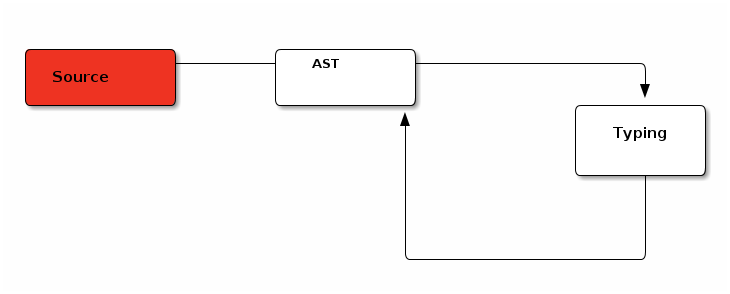
\includegraphics[width=.9\linewidth]{img/phases.png}

\subsection{Typing}
\label{sec-5-2}

This is a separate analysis, made prior to any execution. The interpreter can
be executed in the knowledge that there will be no typing problems during
execution, with the exception of user inputs.

This is made using type-checking rules. The language is strictly
monomorphic and therefore has simple rules.



\subsection{Other analyses}
\label{sec-5-3}

Apart from typing, other small static analyses are already implemented, to be
run prior to the interpretation of the program.


\subsubsection{Unused variables}
\label{sec-5-3-1}

Activating the \texttt{-strict} option will transform the unused variables warnings
into errors.

\subsubsection{Bound checking}
\label{sec-5-3-2}

Out of bounds access for arrays and matrices is checked at run time.

\subsection{Data structures}
\label{sec-5-4}

Should we use hash-mapped tries instead of maps ?

\subsection{Backward compatibility}
\label{sec-5-5}

The \texttt{-old} switch activates the old more lenient behavior if it is needed to
get old version to work.



\section{Conclusion}
\label{sec-6}

We have released a first version of a new interpreter of VisuAlg Portugol,
with stricter type policy.



\section{Future work}
\label{sec-7}

\subsection{Toplevel}
\label{sec-7-1}
\subsection{Visitor}
\label{sec-7-2}
\subsection{Analyses}
\label{sec-7-3}

\subsection{GUI with \texttt{Js\_of\_ocaml} + Static HTML}
\label{sec-7-4}

\subsubsection{Technical notes}
\label{sec-7-4-1}
\begin{itemize}
\item For the CSS, use Bootstrap/ Maybe \texttt{Bootflat}:

\item And \href{http://fortawesome.github.io/Font-Awesome/}{FontAwesome}
\end{itemize}


\subsection{JIT compilation with LLVM}
\label{sec-7-5}
% Emacs 24.3.1 (Org mode 8.2.6)
\end{document}